% 刚体转动数值模拟
% Matlab|数值计算|刚体转动

\pentry{刚体运动方程(四元数)\upref{RBEMQt}, 四阶龙格库塔法\upref{OdeRK4}}

这里给出使用 4 阶龙格库塔法模拟刚体绕固定点转动的 Matlab 代码. 程序中给出的默认参数用于模拟一个初始静止的长方体受到一个 $(1,1,1)$ 方向的大小为 $0.05$ 的恒力矩时的加速转动.

运行结果见\href{http://wuli.wiki/apps/rigBdRot.html}{互动演示}, 截图如\autoref{RBRNum_fig1}.

\begin{figure}[ht]
\centering
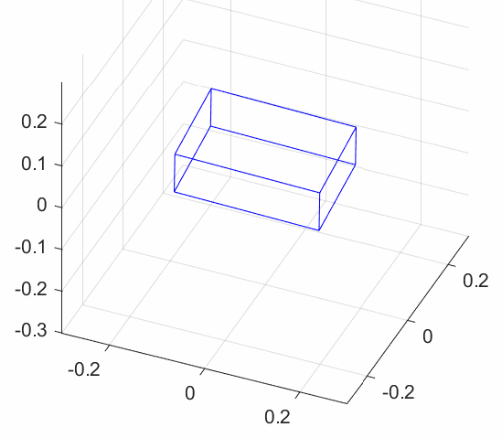
\includegraphics[width=8cm]{./figures/RBRNum_1.png}
\caption{动画截图} \label{RBRNum_fig1}
\end{figure}

为了验证数值解的正确性, 我们在生成动画之前用 \verb|verify| 函数验证角动量定理, 也就是把力矩函数 \verb|tau(t)| 做数值积分, 再与数值解中的角动量进行对比, 结果如\autoref{RBRNum_fig2}.
\begin{figure}[ht]
\centering
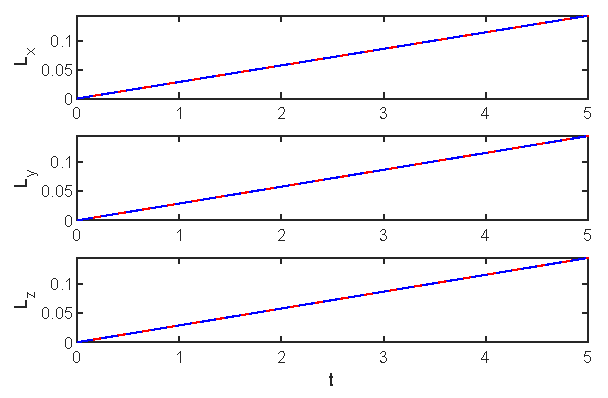
\includegraphics[width=12cm]{./figures/RBRNum_1.pdf}
\caption{验证角动量定理, 三个图分别是角动量的三个分量, 蓝线是力矩积分, 红色是数值解中计算的角动量} \label{RBRNum_fig2}
\end{figure}

\subsubsection{rigBdRot.m}
\begin{lstlisting}[language=matlab]
% 刚体绕固定点转动的数值计算

function rigid_body_rotation
close all;
% === 设置长方体 ===
a = 0.3; b = 0.2; c = 0.1; M = 1; % 边长和质量
I0 = M/12 * diag([b^2 + c^2, a^2 + c^2, a^2 + b^2]); % 惯性张量
w0 = [0; 0; 0]; % 初始角速度
q0 = [1; 0; 0; 0]; % 初始朝向(四元数)
tau = @(t) 0.05*[1; 1; 1]/sqrt(3); % 力矩函数
tmin = 0; tmax = 5; % 起始时间
Nt = 501; % 时间步数
% ================

% 解微分方程
invI0 = inv(I0);
Y0 = [q0; w0];
f = @(Y,t)ode_fun(Y, t, I0, invI0, tau);
[Y, t] = odeRK4(f, [tmin, tmax], Y0, Nt);

% 验证角动量定理
verify(Y, t, I0, tau);

% 播放动画
figure; hold on; grid on; axis equal; view(23, 36);
axis([-0.3, 0.3, -0.3, 0.3, -0.3, 0.3]);
for it = 1:Nt
    q = Y(1:4, it);
    R = quat2mat(q);
    clf; hold on; grid on; axis equal; view(23, 36);
    axis([-0.3, 0.3, -0.3, 0.3, -0.3, 0.3]);
    plot_cube(R, a, b, c);
    title(['t = ' num2str(t(it), '%.3f')]);
    drawnow();
    % 取消注释可将每一帧保存为 png 图片(当前目录下)
    % saveas(gcf, [num2str(it) '.png']);
end
end

% 微分方程求导函数
function dY = ode_fun(t, Y, I0, invI0, tau)
q = Y(1:4); w = Y(5:7);
q = q / norm(q);
R = quat2mat(q);
RT = R';
dw = R*invI0*RT*(tau(t) - cross(w, R*I0*RT*w));
dq = 0.5*quat_mul([0; w], q);
dY = [dq; dw];
end

% 两个四元数相乘
function out = quat_mul(q1, q2)
s1 = q1(1); v1 = q1(2:4);
s2 = q2(1); v2 = q2(2:4);
out = [s1*s2 - dot(v1,v2); s1*v2 + s2*v1 + cross(v1, v2)];
end

% 由四元数 q 求旋转矩阵 R
function R = quat2mat(q)
s = q(1); vx = q(2); vy = q(3); vz = q(4);
R = [1 - 2*vy^2 - 2*vz^2, 2*vx*vy - 2*s*vz, 2*vx*vz + 2*s*vy;
    2*vx*vy + 2*s*vz, 1 - 2*vx^2 - 2*vz^2, 2*vy*vz - 2*s*vx;
    2*vx*vz - 2*s*vy, 2*vy*vz + 2*s*vx, 1 - 2*vx^2 - 2*vy^2];
end

% 画长方体(只用一条线)
function plot_cube(R, a, b, c)
x = [-1,  1,  1, -1, -1,  1,  1, -1] * a/2;
y = [-1, -1,  1,  1, -1, -1,  1,  1] * b/2;
z = [-1, -1, -1, -1,  1,  1,  1,  1] * c/2;
P = R * [x; y; z];
order = [1, 2, 3, 4, 1, 5, 6, 7, 8, 5, 6, 2, 3, 7, 8, 4];
plot3(P(1, order), P(2, order), P(3, order), 'b');
end

% 验证角动量定理
function verify(Y, t, I0, tau)
Nt = numel(t);
L = zeros(3, Nt); % 解的角动量
for it = 1:Nt
    q = Y(1:4, it); w = Y(5:7, it);
    R = quat2mat(q);
    L(:, it) = R*I0*R'*w;
end

L0 = zeros(3, Nt); % 力矩积分的角动量
L0(:, 1) = L(:, 1);
for it = 2:Nt
    L0(:, it) = L0(:, it-1) + ...
        integral(tau, t(it-1), t(it), 'ArrayValued', true);
end

figure;
for i = 1:3
    subplot(3, 1, i);
    plot(t, L(i, :), 'r'); hold on;
    plot(t, L0(i, :), 'b--');
end
subplot(3, 1, 1); ylabel L_x;
subplot(3, 1, 2); ylabel L_y;
subplot(3, 1, 3); ylabel L_z;
xlabel t;
end

% 四阶龙格库塔解微分方程 http://wuli.wiki/online/OdeRK4.html
function [Y,t]=odeRK4(f,tspan,Y0,Nt)
Nvar=numel(Y0);
dt=(tspan(2)-tspan(1))/(Nt-1);
Y=zeros(Nvar,Nt);
Y(:,1)=Y0(:);
t=linspace(tspan(1),tspan(2),Nt);
for ii=1:Nt-1
    K1=f( t(ii),        Y(:,ii)          );
    K2=f( t(ii)+dt/2,   Y(:,ii)+K1*dt/2  );
    K3=f( t(ii)+dt/2,   Y(:,ii)+K2*dt/2  );
    K4=f( t(ii)+dt,     Y(:,ii)+K3*dt    );
    Y(:,ii+1)=Y(:,ii)+dt/6*(K1+2*K2+2*K3+K4);
end
end
\end{lstlisting}
